\chapter{Versioning}
\label{chap:versioning}

Versioning determines creation and management of product versions. The product is what a provider offers to a consumer. A new version of a product can be created when a modification is needed. Consumers can use the same product but they can use its different version. Version can be created to fulfill requirements or due to improvements of functionality. 

Any of new versions of the product mustn't influence the execution of consumers code. When the product is customized, a change has to be compatible with all consumers. In case the change is incompatible, it is needed to produce a new version. Before a consumer switches to the new version, an agreement between provider and consumer has to be established. The consumer then has to do required changes within his functionality.

A change which leads to necessity of modification on consumer side can be a new requirement from one of the consumers. In this case the particular customer can switch to the new version. Other consumers can follow their schedule and switch to the newest version when it is suitable for them. 

In service oriented architecture the services as they are described in Section \ref{sec:services} are the product. Provider is the one who provide services - server. Consumer is the one who use services - client.

\section{Version compatibility}
\label{sec:v-compat}
The changes which can be done within the services can have different impact on consumers. One type does not require changes on client side the other one on the contrary does. Following changes done on the server side there are two forms compatibility of two service versions. \cite{website:service-versioning}
\begin{description}
  \item[Compatible changes] \hfill \\
  Compatible changes are that changes of product which do not affect any existing consumer functionality. Compatible changes are for example implementation bug fixes or additions of parameters in interface to support an implementation modification.
  \begin{enumerate}
    \item[Backward compatible] \hfill \\ 
  When a new version of a service is deployed the consumer of an earlier version must be able to interoperate with the new version without any modification of his application. If a service update, is backward compatible it is compatible with older version of itself. Backward compatible change can be an addition of a new resource or a new capability to the resource. \hfill \\ 
  Example: \hfill \\ 
  Service has action \hfill \\ 
  \begin{lstlisting}
  GET   /customers/{customerId}
  \end{lstlisting}
  and we add a new action to get only the name of a customer with assigned id
  \begin{lstlisting}
  GET   /customers/{customerId}/name
  \end{lstlisting}

  This addition doesn't harm any consumer of the service, because they can continue to use every capability which has been already integrated in their systems. They are is still a part of the new version of the service. 
  
  \item[Forward compatible] \hfill \\
  The service version is forward compatible when it is designed in a way it can support future modifications. It is hard to achieve the forward compatibility because its about unknown future changes which can be done. Services should be designed in a way that they can be modified.
  \end{enumerate}
  
  \item[Incompatible changes] \hfill \\
  Incompatible changes are breaking changes which affect consumers of services. Breaking changes can be performed by adding or removing an enumeration, removing or renaming a global type or element, changing the optionality of an element from optional to required.
  \begin{enumerate} 
    \item[Backward incompatible changes]  \hfill \\
    Backward incompatible changes are changes which break the consumers using an earlier version of service. It means that the new version is no longer compatible with earlier version of itself. It cannot interpret the data of its earlier version or interprets them in wrong manner.
    
    As an example there is a service \emph{customer}. Action POST stores a new customer. The request contains a customer representation in json format: 
    
\begin{lstlisting}
    POST   /customers
    Content-Type: application/json
    
    {
    "Name": "Peter",
    "Surname": "Sun",
    "DateOfBirth": "20 May 1978",
    "Address": {
        "Line1": "Road 23",
        "Line2": "London",
        "PostalCode": "AA0000A"
        }
    }
\end{lstlisting}

If the element \emph{DateOfBirth} is removed from service interface it will be a breaking change. The clients would send requests containing the DateOfBirth element which wouldn't be processable. To use the new version of customers service client have to integrate the changes. 

    \item[Forward incompatible changes] \hfill \\
    These changes break the forward compatibility of the service. It means that a future version won't be compatible with existing one, any modifications of current version don't preserve compatibility.
  \end{enumerate}
\end{description}

\section{Versioning of services}
\label{sec:verioningservices}
Thanks to the versioning services can evolve and can be customized. When a breaking change of a service is implemented the new version can be created so that existing consumers of services are not affected. Release of a new version doesn't remove the previous one. Multiple versions can coexist and can be used at the same time. 

\subsection{Versioning on different levels of a service}
There are three levels of interpretation of a \emph{service} as was already described in Section \ref{subsec:levels-of-service}. A change and consequent creation of a new version can occur within each of this levels - service implementation, service interface and business abstraction.

\subsubsection{Versioning of service implementation}
The implementation of a service can be changed. The new version of service can be either backward compatible or backward incompatible. The implementation is encapsulated below the interface and is not visible for outer world. It can be modified without affecting clients. The backward compatible changes in this level can be a simple bug fix. The incompatible changes are modifications which influence the service calls responses.

Every change which has to be done in the implementation of a service needs to be validated against the contract. When the implementation which is going to be replaced is a breaking change from the point of view of the consumer, agreement with the change of contract is needed. Consequently, new version has to be released.

Changes of the implementation lead to the versioning of the code. Compatible changes can be done without a new version. Having only compatible changes they can be be versioned after specific amount of changes (this amount should be specified as a part of versioning strategy) for proper change management. In case of a breaking change, code has to be versioned.

\subsubsection{Versioning of service interface}
Service interface is an entry point for consumers to work with the services. Interface can be versioned as well and its change impacts the consumer application. Compatible change of the interface is an addition of an action. On the other side non compatible change is a removal of an action. When a new action is added, no one is using it and it is optional if somebody would make use of it. When an action is removed, consumers which are using it are negatively affected and their implementation can be broken.

\subsubsection{Versioning of business service}
Sometimes it is needed to change the business service. It means the business which is abstracted have to be changed. For example because of new requirements due to legislative a business service needs modifications. If this kind of change affects behaviour, semantic or functionality of existing service, it is easier to create a new service rather than a new version. 


\subsubsection{Conclusion}
\emph{Service interface versioning} is the interpretation which will be further described and analyzed. It brings various approaches with their advantages and disadvantages. The versioning of services is quite young topic and there are still very vibrant discussions about the best approach.

\section{Versioning strategy}
\label{sec:version-strategy}
There is a need to specify a set of rules to version services consistently. Those rules form the versioning strategy. They are related to new service version release and access or number of accessible version at the same time. The rules are the matter of SOA governance. There isn't single correct way to govern the service versioning. Defined strategies should be followed and practiced during whole service lifecycle \cite{soa-governance}:

\begin{description}
  \item[Strict]  \hfill \\
  Any change of a service results in a new version as shown on the Figure \ref{fig:strict-strategy}. This strategy does not support backward or forward compatibility because every modification results in a new version. This approach is the safest one and can be in place when there is a sensitive data exchange between two organizations. Consumer organization have a control over the services evolution. If any change is done the service version increases and client has to integrate it. 
    
\begin{figure}[htp] \centering{
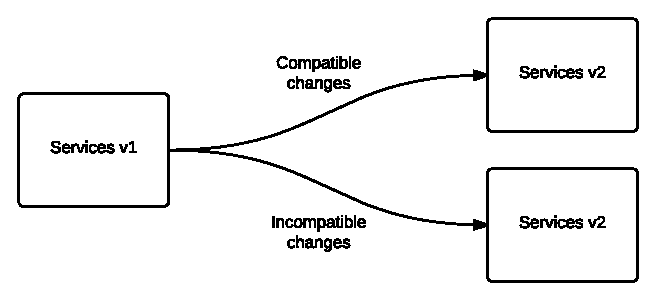
\includegraphics[width=8cm]{img/strict-strategy.pdf}}
\caption{Strict strategy versioning}
\label{fig:strict-strategy}
\end{figure} 

  \item[Flexible] \hfill \\
  Any incompatible changes result in a new version and the service design supports backward compatibility (Figure \ref{fig:flexible-strategy}). This is common approach. Changes which are backward compatible modify the service interface without affecting the service version. They are considered safe and do not impact any client.
  \item[Loose] \hfill \\
  Any incompatible changes result in a new version and the service design supports backward and forward compatibility. The strategy is similar to Flexible one. Incompatible changes results in a new version(Figure \ref{fig:flexible-strategy}). The difference is in supporting this designed so that it a forward compatible changes. Service interface is designed so that the future changes can be added without a breaking change.
\end{description}

\begin{figure}[htp] \centering{
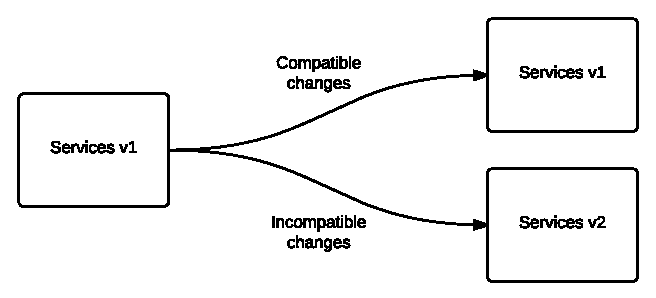
\includegraphics[width=8cm]{img/flexible-strategy.pdf}}
\caption{Flexible and Loose strategy versioning}
\label{fig:flexible-strategy}
\end{figure} 

The strategy needs to be determined during the analysis stage of application lifecycle. It includes more decisions regarding versioning which have to be done before the service implementation such as version identification by digits or version lifecycle.

\subsection{Version identifiers}
\label{subsec:versionid}
Version Identification is one of the fundamental \gls{design-patterns}. Version is indicated by decimals separated by periods. The version number length and meaning of the digits should be established as a part of the versioning strategy. Every digit increments accordingly to significance of the change. Full version number is usually composed from two to four digits X.Y.Z.R.

Explanation of the digits \cite{soa-governance}:

\begin{enumerate}
  \item[Major changes X] \hfill \\
  Major changes are non-backward compatible changes. After a major change, new service interface is no longer compatible with the old one. These changes break the usage of the service by the consumer. They are imposed to the new version and consumers need to adjust their programs to switch to this version. 
  
    \item[Minor changes Y] \hfill \\
  Minor changes are backward-compatible changes. The changes do not impact consumers, the new version continue to support the consumers working with the old version. Examples can be new optional element to existing type, a change of optionality of a local element from required or optional, adding global type or global element, etc.
  
  \item[Patch version Z] \hfill \\  
  Patch version Z is incremented if only backwards compatible bug fixes are introduced. A bug fix is defined as an internal change that fixes incorrect behavior.
  
  \item[Revisions R] \hfill \\ 
  Revisions are changes without semantic content, for example formatting, comments, etc. They do not affect the functionality of the service and service consumers.
\end{enumerate} 

Using version identifiers to express the compatibility by incrementing major and minor numbers serves to guarantee compatibility. There is another approach to indicate the version of services related to amount of work. The number increment according to effort which have been dedicated to the change. The big effort increments the major number and modest effort the minor number. This two approaches can be combined and in most cases they are, preserving mainly the compatibility guarantee and less often communicating the effort made. \cite{soa-governance}


\subsection{Service version life-cycle}
Service life-cycle defines the time period in which a version should be maintained. When the time is short, customers don't have enough time for their upgrades required in order to switch to the new version. On the other hand when the period is too long, too many versions of service have to be maintained. The suitable time span is a result of consideration of each individual organization with respect to their capability to deal with changes.

Product version should be always compatible with consumers usage. When a new version of the service method is released, it is needed to have the old one present in the implementation. If any of the consumers use it. When the service method is going to be replaced by new one, both versions have to be held to not impact any consumer. The older version can be marked as deprecated, which doesn't influence its usage from the point of view of the consumer. But means that provider waits until all consumers switch to the newer service version. When the deprecated method is no longer used, it can be safely removed. 

%This lifecycle is possible only when the service method versioning approach is implemented, in case of whole-service versioning, when the service is given into state deprecated, it is equivalent to its removal. New agreement between the provider and consumer is needed, so that consumer have to implement changes to use the new service. %or just keep using the older version. The whole-service versioning provides less flexibility.


\section{Versioning approaches}
\label{sec:versioning-approaches}

The service interface can be versioned in multiple ways. One of the approaches is deployment of new version to new environment. This approach is widely used for code versioning not only for services. Other approach is specific for service interface versioning. Multiple versions can coexist at the same time. Then there arises a question how a consumer can access the requested version of the service. The possibilities of access them is analyzed in Chapter \ref{chap:versionaccess}.


\subsection{New version - new environment approach}

The versioning is based on deploying a new version of \gls{api} to a new environment. The deployment process is identical to software deployment. Service changes are deployed on a new environment. %incrementing the API version number.

\subsubsection{Version identification}
When in an API with version \emph{v1} a change is done, implementation version number is incremented in minor digit. From the definition in Section \ref{subsec:versionid}, it is obvious that this is backward compatible change. The implementation than gains for example identifier \emph{1.1}. The services do not change their interface and their consumers are not affected. 
When there is a breaking change or there is a specified number of changes or amount of work done, API version increments and it is released to a new environment. 

The API version increase in major identifier to \emph{v2} because non-backward compatible changes were done. Consumers of services need to do required changes to use newer version of services. Than they call services using new environment. 
The API is usually marked by a major identifier so that \emph{API v1} or\emph{API v2} and so on.
The implementation of API is versioned using minor, path and revision identifiers. The implementation which is deployed on the server than can have a version for example \emph{1.0.0.0} or \emph{1.3.1.2}. The number increases depending on what kind of changes was done on the implementation.

Figure \ref{fig:version-identifying} shows an expamle of identification of version. Implementations of the version are identified by 4 digits. Last three of them are increasing within one version of service API. After a breaking change a new API version is created with incremented version number. 

\begin{figure}[htp] \centering{
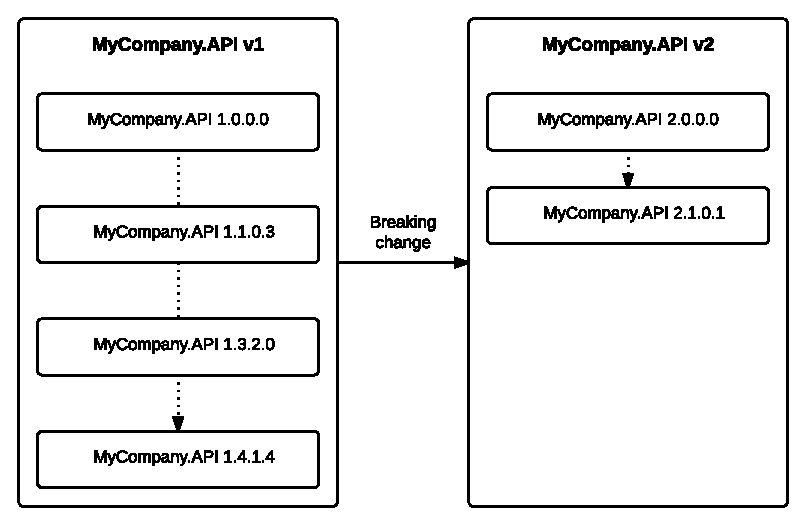
\includegraphics[width=8cm]{img/version-identifying.pdf}}
\caption{Incrementation of version identifiers}
\label{fig:version-identifying}
\end{figure} 


\subsubsection{Deployment principles}
The deployment goal is to deliver a high quality product to the consumer. How to reach it is responsibility of deployment management and their strategy. The ideal state is when the deployment is simple and fast. To obtain this the changes deployed should be small and should happen often and the new version should be well tested before deployment to production environment.

\subsubsection{Environments}
To get a good quality API, it is quite necessary to have more than one environment running the same version of API. Every environment has its role. There are at least two of them - development and production. Development environment is one with the latest version of API and production environment contains a stable version of API used by consumers.

Better is to have more than just two environments. There should be at least one environment dedicated to testing and one environment can hold a stable version version of API from which runs the releases to production environment. The last one is generally named as staging environment. It simulates the production environment so that provides to producer test environment where the API is running. It can discover system failures before the main release to the production. On Figure \ref{fig:environments} is shown the possible composition od environments.

\begin{figure}[htp] \centering{
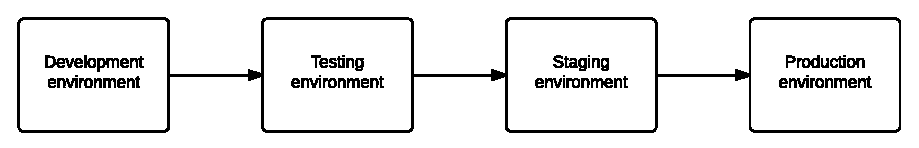
\includegraphics[width=10cm]{img/environments.pdf}}
\caption{Environments architecture}
\label{fig:environments}
\end{figure} 

One environment (server) holds just one version of API. If another version is needed to be available it has to be deployed on another server. Then customers are using different servers, as shown on the image \ref{fig:consumer-server}

\begin{figure}[htp] \centering{
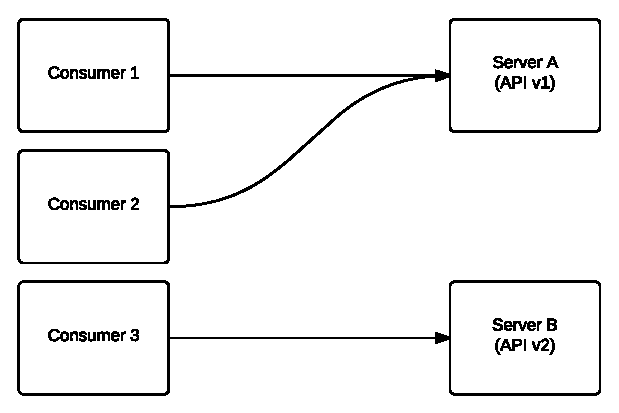
\includegraphics[width=8cm]{img/consumer-server.pdf}}
\caption{Possible usage of two deployed versions of API}
\label{fig:consumer-server}
\end{figure} 

\subsubsection{Deployment strategy}
One of the approaches how to release a new version of API is cutover, the other one is parallel development. The cutover requires downtime period planning. The downtime determines when a cutover occurs. 

The parallel deployment allow to have more versions on which the development, testing and consuming are proceeding (Figure \ref{fig:parellel-development}). This approach offers more reliability, because of running backup system but requires more effort from provider and consumers. When a new version is going to be released, it is deployed to environment but keeping the old system running on its environment and continue with development, support and usage of the old one. 

\begin{figure}[htp] \centering{
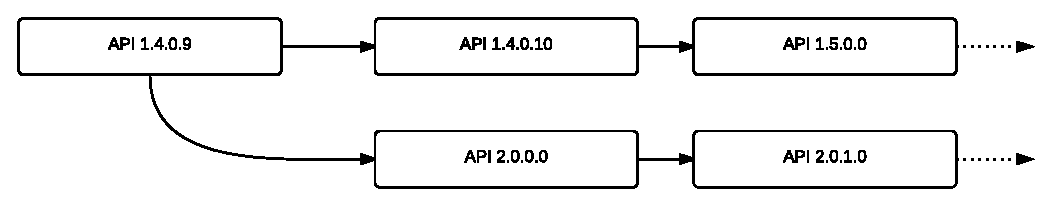
\includegraphics[width=8cm]{img/parellel-development.pdf}}
\caption{Parallel development}
\label{fig:parellel-development}
\end{figure} 

Having cutover approach when the actual version of API on the development environment is going to be emitted to the production the developed code version number increases (Figure \ref{fig:cutover-development}). Development on a new version starts. The cut version is, after being stable, released to the production. Consumers connect to production environment to use services. 

\begin{figure}[htp] \centering{
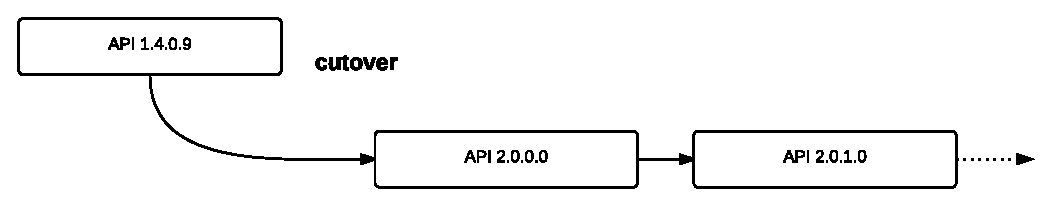
\includegraphics[width=8cm]{img/cutover-development.pdf}}
\caption{Cutover development}
\label{fig:cutover-development}
\end{figure}  


\subsubsection{Deployment methods}
There are more possibilities how to deploy the API to an environment. The whole API can be copied and deployed, it can be used a third party tool to manage deployments or it can be automated by creation of an installer.

\begin{description}
  \item{File copy method} \hfill \\
  The API image is copied to a new environment manually. This method is network based and provide diminution of distribution time and assistance in updates. On the other hand there can be problems with accessing the files on network and other with determining the reason of possible system fails. 
  \item{Continuous integration method} \hfill \\
  The \gls{scm} (SCM) to assist the distribution of the system. SCM server contains the master version of the API, developers work with its local version and after making some changes they push them to the server. Having the most recent version depends just on simple update from SCM server to get the last revision (what is revision was explained in Section \ref{subsec:versionid}). The SCM tool has a history of changes within a files. Developers can see every change done on the file from its creation to its newest version. When a change causes a failure of function of software, it can be reverted.
  
  With the SCM is connected a practice called Continuous Integration (CI). When someone push a change of a file to the SCM, the continuous integration ensures the build process and testing of whole project. The new change is integrated into the implemenation. If the CI build or tests fails it is possible to see which file caused the failure. 
  Result of the build process is a \ref{dll} file. This file is deployed to environments. Whole process is shown on Figure \ref{fig:deployment-process}.
  
\begin{figure}[htp] \centering{
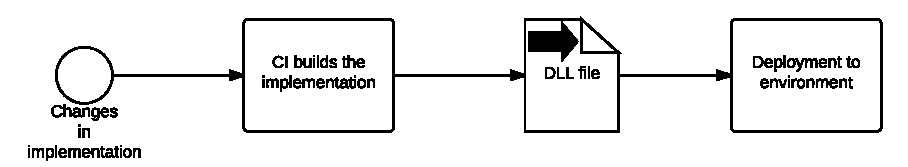
\includegraphics[width=11cm]{img/deployment-process.pdf}}
\caption{Contunuous Integration and DLL deployment}
\label{fig:deployment-process}
\end{figure} 
   
  \item{Installer method} \hfill \\
  Both of the methods above requires the more of the user effort. This method is more automate. It allows installer technology integration by creating installer package which is distributed and easy to use. Aside this benefits this methods struggles with the minor changes distribution because the installation package has to be rebuilt.
\end{description}


\subsubsection{Access to versions}
Consumers are always calling just one version of the API service. The one which is deployed to the targetted environment. They can switch she version of API only after deployment of new version on their production environment.

\subsubsection{Advantages and disadvantages}
Advantage of this approach is the access to API. He has accessible one version of API at the same time.

The main disadvantage of this approach is the incapability of easily repair issues in a previous version of the API. When the API is in versions up to \emph{v3} in development environment and in versions \emph{v1} and \emph{v2} in production environment. When an error is found in production in \emph{v1} (Figure \ref{fig:bug-in-previous-version}) this bug is probably supposed to be present also in later versions \emph{v2} and \emph{v3}. Then the bug has to be fixed in all three versions and redeployed on servers which is usualy not a trivial operation.

\begin{figure}[htp] \centering{
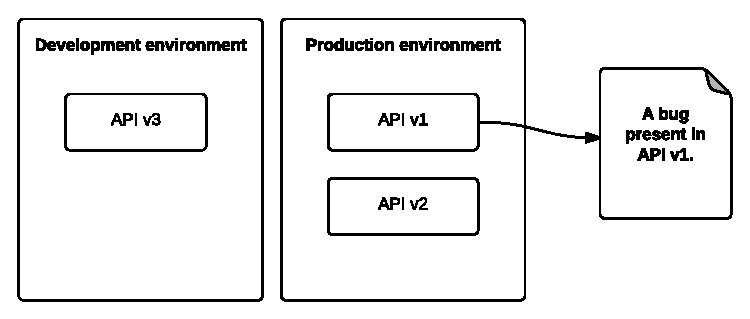
\includegraphics[width=11cm]{img/bug-in-previous-version.pdf}}
\caption{An error found in one of the previous version}
\label{fig:bug-in-previous-version}
\end{figure} 

\bigskip


\subsection{Service interface versioning approach}

Another approach to versioning is more than one version of the service API running at the same time. This approach can be implemented using various principles. \emph{Service interface versioning} is the interpretation which will be further described and analyzed. It brings different principles of how to be accessed. Version access appraches will be explained in Chapter \ref{chap:versionaccess}.

This versioning approach allows to make changes to the API and release its new version without waiting for consumers to integrate the changes. All versions can run concurrently and be accessed by clients. When there are two coexistent versions of API, \emph{v1} and \emph{v2}, consumer has access to both of them. According to what he sent in the request he is directed to the correct version. Each of these versions can be on the same environment, or can be separated. This concept is invisible to  consumers.

%Each version has its own implementation and is distinguishably addressed.

%Versioning management of services requires the proper definition of following concepts \cite{website:versioning-in-soa}:
%what will be versioned and how, the life-cycle of the versions and the access to the version.
%\begin{enumerate}
 % \item Units of versioning
 % \item Service changes, constituting a new version
 % \item Service version life-cycle considerations
 % \item Version deployment/access approaches
%\end{enumerate}

\subsubsection{Units of versioning}
\label{sec:units}

The service layer of an application developed by a provider is an \emph{API} containing \emph{services}. Services contain \emph{methods (actions)} which allows to manipulate with the resources. The relationship between these entities is shown on Figure \ref{fig:service-layer-design}

\begin{figure}[htp] \centering{
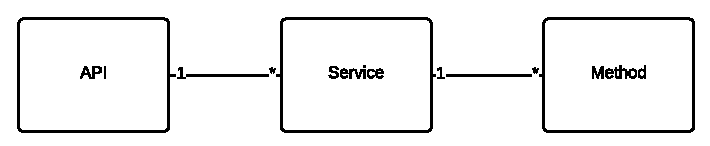
\includegraphics[width=11cm]{img/service-layer-design.pdf}}
\caption{Design of service layer}
\label{fig:service-layer-design}
\end{figure} 

There are three possibilities of what can be versioned in service interface - API, services or service methods. Relationship between those possibiliteies is shown in Figure \ref{fig:service-layer-design}. 

The granularity of versioning can be defined by the change which is the reason of creating of a new version. If the change happens just in changes it is possible to version just the method on the other hand when a set of services are changed the whole API should be versioned. These are not rules but the decision what to version should be originated in versioning strategy. The three options can be interchanged should be done carefully to don't complicate services architecture.

Version identified by number which is typically just major digit for each of the version unit. For example the API can be in version \emph{v2} and can contain a service with version \emph{v1} and \emph{v2}, this service versions can have a method of versions \emph{v1} and \emph{v2}.

/obrazok

\begin{description}
\item{Versioning of API} \\
The API containing all services can be versioned. Having the version \emph{v1} API is incremented to version \emph{v2}. This new version can be deployed on the same environment which was running the API v1. Consumers can access them both. Change of API influences every consumer.
\item{Versioning of service} \\
  The whole service is versioned with all its methods. Versioned service with version \emph{v1} is changed to \emph{v2}. It can be still part of the API \emph{v1}, just the service version is incremented. When the new version on the service is deployed on environment both service versions can be accessed. The changes influences just consumers which were using the service.
\item{Versioning of service method} \\
  In most cases the change arises just in a method or some methods of a service. It is not necessary to version the whole service, but there is an option to version just these operations. \\
  The benefits of this approach are less code which is deployed because just a changed methods are redeployed in a new version. Services remain unchanged, their name and classification, when there is a method added. The changes concern just a consumers which use the method, instead of consumers of the service containing changed method. \\
  When the versioning of method is used it is needed to deploy each method with its own endpoint address, the advantage is that the \gls{sla} is provided for the method so that it is not changed the SLA of the same service.\\
  Moreover the addressing schema becomes more complex, the consumer has to specify not just the service but also the method and version of method which wants to use.
  In spite of the more elaborate routing this possibility of versioning offers more flexibility. It adapts the services versioning to versioning practices of commonly used programming languages. \\
Other benefit of this versioning unit adding and removing of methods in a service. New method new can be added without any impact on existing consumer. Regarding the removal of a method, there is a deprecation concept. A method which has been for example replaced by new version can be signed as deprecated. A deprecated method takes part until there are still consumers which are using it. When all consumers stop to use it the method can be removed.\\
  Version of changed method \emph{v1} increase in \emph{v2}, this method can be for example part of the service of \emph{v2} and API \emph{v1}.
\end{description}

\subsubsection{Logic of service versioning}
There is a version of the API which is already used in production when there is a breaking change the implementation of new version of API is integrated with the old one. Both version can be deployed into production, it is not mandatory they are on the same environment. Consumer can continue to use the old version and after integrating the changes whenever he can switch the version. It is needed to be clear in advance where the version will be places and how will be accessed.
Depending on the principle of accessing the version there can be said explicitly in endpoint address (URL) which version of API, service or method is called. The request is directly roated to requested version. The other approach to have the same endpoint address for each version of the versioned unit and the routing than pass through an intermedia which resolves the correct version, decision is based on one of the parameters send in request. Option of accessing the version will be described in Chapter \ref{chap:versionaccess}.

\subsubsection{Environments}
There are multiple ordered environment beginning with the development and ending with production, same as in the implementation versioning (new version has always new environment) described above. The number and importance of environment is a question of development strategy. For example there can be development environment, some test environments, staging and production environment. 

/todo
parallel development
version lifecycle, how long to maintain the version

\subsubsection{Advantages and disadvantages}
The advantage is the version access at any time after deployment in production, the process in not dependent on consumers integration. The other very significant advantage is the fixing of failures, ???
On customer site the disadvantage is the forcing to add the version identification in the requests, he has to change it everytime he change the version of API or its subunits. For provider it is needed to implement a logic of access different versions.
/TODO



%\subsection{Version definition}
%It is necessary to analyze the services/methods from the point of view of changes, their impact on the consumer. Analysis of possible changes deals with influence of change on the consumers execution and consequently defines the changes which will break it. When the change of the service or method is breaking it leads to the creation of new version.

%The components of the service are interface and message, both of them could be changed and cause the release of new version.

%\subsubsection{Interface changes}
%A change of interface has significant impact on the consumer, it requires many modification of customers implementation or even completely new service. The deprecation of a method is equivalent to its removal and should occur rarely.
%When following semantic messages model, the interface is never changed. Advantage of this approach has source in the fact that all changes can be done just within the methods of service. 
%When the methods are units of versioning they are deployed individually and new methods can be added without any impact on existing consumer. When the method is going to be removed, it is first deprecated, so that is still kept around the service and could be used until all consumers stop to use it. The changes are contained in messages and are not shown within the interface.
%Than as seen it is better to design the versioning definition in order to not include the interface changes.



%\subsubsection{Message changes}
%When using the semantic message model the changes of service interface do not change the interface itself but are contained in message. The message is created by a schema which describes its content. Changes in schema can provide different cases of compatibility with actual implementation and can be divided in three categories:

%\subsection{Version access}
%It is needed to define how different consumers of services are accessing its version of the service. There are several approaches everyone has its pros and cons. The access possibilities are described in separate chapter \ref{chap:versionaccess}.

%\section{Versioning service implementation}
%Besides versioning the service interface, it is possible to consider an implementation. The underlying implementation can changed without affecting the interface itself. 

